\documentclass[11pt,a4paper]{article}
\usepackage[T1]{fontenc}
\usepackage[utf8]{inputenc}
\usepackage{lmodern}
\usepackage{textcomp}
\usepackage[left=1.8cm,right=1.8cm,top=2.3cm,bottom=2.2cm,headheight=14pt,headsep=8pt]{geometry}
\usepackage{multicol}
\usepackage{xcolor}
\usepackage{fancyhdr}
\usepackage{graphicx}
\usepackage{array}
\usepackage{amsmath,amssymb}
\usepackage{setspace}
\usepackage{longtable}
\graphicspath{{../}}
\definecolor{ygreen}{RGB}{46,139,87}
\renewcommand{\normalsize}{\fontsize{10.9}{13.4}\selectfont}
\renewcommand{\familydefault}{\rmdefault}
\setlength{\parindent}{0pt}
\setlength{\columnsep}{0.8cm}
\setlength{\columnseprule}{0.4pt}
\setlength{\multicolsep}{3pt plus 1pt minus 1pt}
\renewcommand{\textsubscript}[1]{\ensuremath{_{\text{\fontsize{8}{8}\selectfont #1}}}}
\renewcommand{\textsuperscript}[1]{\ensuremath{^{\text{\fontsize{8}{8}\selectfont #1}}}}
\newcommand{\diqqat}[1]{\par\smallskip\noindent\textbf{Diqqat!} #1\par\medskip}
\newcommand{\javob}{\par\smallskip\noindent\textbf{Javob:} \rule[-2pt]{7.5cm}{0.4pt}\par\smallskip\noindent\textbf{Diqqat!} Javobingizni javoblar varaqasiga ko`chirib yozing.\par\medskip}
\pagestyle{fancy}
\fancyhf{}
\renewcommand{\headrulewidth}{0.4pt}
\fancyhead[L]{\textit{Milliy sertifikat 2026. Kimyo}}
\fancyhead[R]{3-variant}
\fancyfoot[L]{\fontsize{8}{9}\selectfont \textcopyright{} Colba maktabi, 2026}
\fancyfoot[C]{\thepage}
\fancypagestyle{first}{\fancyhf{}\renewcommand{\headrulewidth}{0pt}\fancyfoot[L]{\fontsize{8}{9}\selectfont \textcopyright{} Colba maktabi, 2026}\fancyfoot[C]{\thepage}}
\begin{document}
\normalsize
\thispagestyle{first}
\noindent\fcolorbox{ygreen}{white}{\parbox{\dimexpr\linewidth-2\fboxsep-2\fboxrule\relax}{%
\textbf{\fontsize{13}{15}\selectfont Nazorat testi}\ \textit{\fontsize{10}{12}\selectfont $\cdot$ Aralash test $\cdot$ 3-variant}\hfill
\begin{tabular}[t]{@{}r@{}}\textit{Milliy sertifikat 2026. Kimyo}\\ \textbf{\textit{\fontsize{8}{9}\selectfont Vaqt:}} \textit{\fontsize{10}{12}\selectfont 180 daqiqa}\end{tabular}}}
\par\medskip
\noindent\textit{Davriy jadvaldan foydalanish mumkin.}
\par\medskip
\begin{multicols}{2}
\noindent\textbf{1.} Quyidagi elementlardan qaysi birining atomida elektronning ``sakrashi'' ro`y beradi?

\noindent A)~\textsl{Ca} \hfill B)~\textsl{Zn} \hfill C)~\textsl{Cr} \hfill D)~\textsl{Fe}\par
\vspace{4pt}
\noindent\textbf{2.} CH\textsubscript{2}=CH--C$\equiv$CH molekulasidagi $\sigma$ va $\pi$ bog`lar \textbf{sonini aniqlang.}

\noindent A)~\textsl{8 va 2} \hfill B)~\textsl{7 va 3} \hfill C)~\textsl{6 va 3} \hfill D)~\textsl{7 va 2}\par
\vspace{4pt}
\noindent\textbf{3.} 0,5 mol sirka kislota eritilgan eritmada 0,49 mol dissotsilanmagan molekula qoldi. Kislotaning dissotsilanish \textbf{darajasini (\%) aniqlang.}

\noindent A)~\textsl{0,2} \hfill B)~\textsl{2} \hfill C)~\textsl{1} \hfill D)~\textsl{5}\par
\vspace{4pt}
\noindent\textbf{4.} pH = 2 bo`lgan HCl eritmasining 100 ml siga pH = 12 bo`lgan NaOH eritmasidan 100 ml qo`shildi. Hosil bo`lgan eritmaning pH \textbf{qiymatini aniqlang.}

\noindent A)~\textsl{2} \hfill B)~\textsl{12} \hfill C)~\textsl{7} \hfill D)~\textsl{9}\par
\vspace{4pt}
\noindent\textbf{5.} Na\textsubscript{2}SO\textsubscript{4} eritmasi inert elektrodlar yordamida 2 A tok kuchi bilan 9650 s elektroliz qilindi. Katod va anodda ajralgan gazlarning umumiy \textbf{hajmini (l, n.sh.) aniqlang.}

\noindent A)~\textsl{1,12} \hfill B)~\textsl{2,24} \hfill C)~\textsl{4,48} \hfill D)~\textsl{3,36}\par
\vspace{4pt}
\noindent\textbf{6.} 28,6 g Na\textsubscript{2}CO\textsubscript{3}$\cdot$10H\textsubscript{2}O 200 g suvda eritildi. Eritmadagi Na\textsubscript{2}CO\textsubscript{3} ning massa \textbf{ulushini (\%) aniqlang.}

\noindent A)~\textsl{5,3} \hfill B)~\textsl{4,64} \hfill C)~\textsl{10,6} \hfill D)~\textsl{3,7}\par
\vspace{4pt}
\noindent\textbf{7.} \textsuperscript{238}\textsubscript{92}\textit{U} atomi 8 ta $\alpha$-zarra va 6 ta $\beta$\textsuperscript{$-$}-zarra chiqarib parchalansa, qaysi izotop hosil bo`ladi?

\noindent A)~\textsl{\textsuperscript{206}\textsubscript{82}Pb} \hfill B)~\textsl{\textsuperscript{206}\textsubscript{80}Hg} \hfill C)~\textsl{\textsuperscript{208}\textsubscript{82}Pb} \hfill D)~\textsl{\textsuperscript{206}\textsubscript{76}Os}\par
\vspace{4pt}
\noindent\textbf{8.} Tarkibida 9,03$\cdot$10\textsuperscript{23} ta molekula bo`lgan ammiak (NH\textsubscript{3}) ning \textbf{massasini (g) aniqlang.} (N\textsubscript{A} = 6,02$\cdot$10\textsuperscript{23})

\noindent A)~\textsl{51} \hfill B)~\textsl{17} \hfill C)~\textsl{8,5} \hfill D)~\textsl{25,5}\par
\vspace{4pt}
\noindent\textbf{9.} CO va CO\textsubscript{2} dan iborat 11,2 l (n.sh.) aralashmaning massasi 18 g. Aralashmadagi CO ning \textbf{massasini (g) aniqlang.}

\noindent A)~\textsl{5,6} \hfill B)~\textsl{11} \hfill C)~\textsl{14} \hfill D)~\textsl{7}\par
\vspace{4pt}
\noindent\textbf{10.} KCl va NaCl eruvchanligining haroratga bog`liqligi grafikda berilgan.
\begin{center}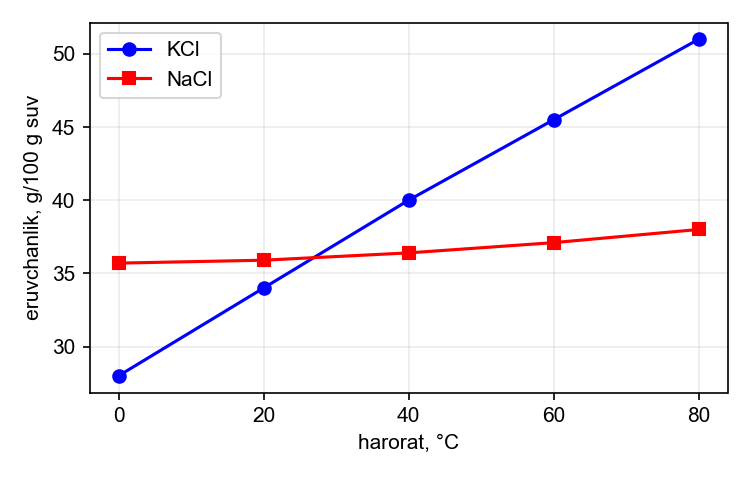
\includegraphics[width=0.86\linewidth]{rasmlar/gen/s2_v03.png}\end{center}
40 \textdegree{}C da qaysi tuzning eruvchanligi katta?

\noindent A)~\textsl{KCl} \hfill B)~\textsl{KNO\textsubscript{3}} \hfill C)~\textsl{NaCl} \hfill D)~\textsl{NH\textsubscript{4}Cl}\par
\vspace{4pt}
\noindent\textbf{11.} 2NO + O\textsubscript{2} $\rightleftarrows$ 2NO\textsubscript{2} + Q muvozanatni o`ngga siljitadigan \textbf{o`zgarishlarni toping}: 1) haroratni oshirish; 2) bosimni oshirish; 3) O\textsubscript{2} qo`shish; 4) katalizator qo`shish.

\noindent A)~\textsl{1, 2} \hfill B)~\textsl{2, 3} \hfill C)~\textsl{1, 4} \hfill D)~\textsl{3, 4}\par
\vspace{4pt}
\noindent\textbf{12.} 3Cu + 8HNO\textsubscript{3}(suyult.) $\to$ 3Cu(NO\textsubscript{3})\textsubscript{2} + 2NO + 4H\textsubscript{2}O reaksiyada 6 mol mis erisa, oksidlovchi vazifasini bajargan HNO\textsubscript{3} ning miqdori necha mol bo`ladi?

\noindent A)~\textsl{12} \hfill B)~\textsl{4} \hfill C)~\textsl{16} \hfill D)~\textsl{8}\par
\vspace{4pt}
\noindent\textbf{13.} 0 \textdegree{}C va 202,6 kPa bosimda 5,6 l gazning massasi 22 g. Gazning molyar \textbf{massasini (g/mol) aniqlang.}

\noindent A)~\textsl{28} \hfill B)~\textsl{32} \hfill C)~\textsl{44} \hfill D)~\textsl{22}\par
\vspace{4pt}
\noindent\textbf{14.} 2,3 g natriy va 3,9 g kaliydan iborat aralashma suvda eritilganda ajralgan vodorodning \textbf{hajmini (l, n.sh.) aniqlang.}

\noindent A)~\textsl{1,12} \hfill B)~\textsl{4,48} \hfill C)~\textsl{3,36} \hfill D)~\textsl{2,24}\par
\vspace{4pt}
\noindent\textbf{15.} Alyuminiy va magniydan iborat 5,1 g aralashma mo`l xlorid kislotada eritilganda 5,6 l (n.sh.) vodorod ajraldi. Aralashmadagi alyuminiyning massa \textbf{ulushini (\%) aniqlang.}

\noindent A)~\textsl{40} \hfill B)~\textsl{52,9} \hfill C)~\textsl{47,1} \hfill D)~\textsl{60}\par
\vspace{4pt}
\noindent\textbf{16.} Cu va CuO dan iborat 14,4 g aralashma mo`l suyultirilgan H\textsubscript{2}SO\textsubscript{4} da ishlandi, 6,4 g qattiq qoldiq qoldi. Hosil bo`lgan tuz \textbf{massasini (g) aniqlang.}

\noindent A)~\textsl{8} \hfill B)~\textsl{25} \hfill C)~\textsl{32} \hfill D)~\textsl{16}\par
\vspace{4pt}
\noindent\textbf{17.} 0,05 mol Ca(HCO\textsubscript{3})\textsubscript{2} tutgan suv qaynatilganda ajralgan CO\textsubscript{2} ning \textbf{hajmini (l, n.sh.) aniqlang.}

\noindent A)~\textsl{0,56} \hfill B)~\textsl{5} \hfill C)~\textsl{2,24} \hfill D)~\textsl{1,12}\par
\vspace{4pt}
\noindent\textbf{18.} Qaysi qatorda faqat amfoter oksidlar keltirilgan?

\noindent\begin{tabular}{@{}p{0.47\linewidth}@{}p{0.47\linewidth}@{}}
A)~\textsl{Cr\textsubscript{2}O\textsubscript{3}, CrO\textsubscript{3}, FeO} & B)~\textsl{CaO, Al\textsubscript{2}O\textsubscript{3}, ZnO} \\
C)~\textsl{ZnO, Al\textsubscript{2}O\textsubscript{3}, Cr\textsubscript{2}O\textsubscript{3}} & D)~\textsl{ZnO, CrO, MgO} \\
\end{tabular}\par
\vspace{4pt}
\noindent\textbf{19.} Cu $\to$ CuO $\to$ CuSO\textsubscript{4} $\to$ Cu(OH)\textsubscript{2} $\to$ CuO o`zgarishlar zanjirida oxirgi bosqichda 8 g CuO hosil bo`ldi. Dastlabki mis \textbf{massasini (g) aniqlang.}

\noindent A)~\textsl{6,4} \hfill B)~\textsl{8} \hfill C)~\textsl{3,2} \hfill D)~\textsl{12,8}\par
\vspace{4pt}
\noindent\textbf{20.} C\textsubscript{6}H\textsubscript{14} tarkibli alkanning nechta izomeri bor?

\noindent A)~\textsl{4} \hfill B)~\textsl{6} \hfill C)~\textsl{5} \hfill D)~\textsl{3}\par
\vspace{4pt}
\noindent\textbf{21.} 5,4 g butadiyen-1,3 ga mo`l brom ta'sir ettirilib, 1,4-birikma mahsuloti olindi. Mahsulot \textbf{massasini (g) aniqlang.}

\noindent A)~\textsl{21,4} \hfill B)~\textsl{43,2} \hfill C)~\textsl{16} \hfill D)~\textsl{10,7}\par
\vspace{4pt}
\noindent\textbf{22.} 9,2 g toluol KMnO\textsubscript{4} ning sulfat kislotali eritmasi bilan oksidlanib, 80\% unum bilan benzoy kislota hosil qildi. Kislota \textbf{massasini (g) aniqlang.}

\noindent A)~\textsl{6,1} \hfill B)~\textsl{7,8} \hfill C)~\textsl{12,2} \hfill D)~\textsl{9,76}\par
\vspace{4pt}
\noindent\textbf{23.} 9,2 g glitserin mo`l natriy bilan reaksiyaga kirishganda ajralgan vodorodning \textbf{hajmini (l, n.sh.) aniqlang.}

\noindent A)~\textsl{3,36} \hfill B)~\textsl{2,24} \hfill C)~\textsl{4,48} \hfill D)~\textsl{1,12}\par
\vspace{4pt}
\noindent\textbf{24.} 5,8 g propanon nikel katalizatori ishtirokida vodorod bilan to`liq qaytarildi. Hosil bo`lgan spirt \textbf{massasini (g) aniqlang.}

\noindent A)~\textsl{6} \hfill B)~\textsl{3} \hfill C)~\textsl{5,8} \hfill D)~\textsl{7,4}\par
\vspace{4pt}
\noindent\textbf{25.} 4,6 g chumoli kislota Ag\textsubscript{2}O ning ammiakli eritmasi bilan to`liq oksidlanganda ajralgan kumush \textbf{massasini (g) aniqlang.}

\noindent A)~\textsl{43,2} \hfill B)~\textsl{10,8} \hfill C)~\textsl{21,6} \hfill D)~\textsl{5,4}\par
\vspace{4pt}
\noindent\textbf{26.} 88,4 g triolein nikel katalizatori ishtirokida to`liq gidrogenlanganda sarflangan vodorod \textbf{hajmini (l, n.sh.) aniqlang.}

\noindent A)~\textsl{4,48} \hfill B)~\textsl{6,72} \hfill C)~\textsl{13,44} \hfill D)~\textsl{2,24}\par
\vspace{4pt}
\noindent\textbf{27.} 34,2 g maltoza to`liq gidrolizlandi va hosil bo`lgan mahsulot Ag\textsubscript{2}O ning ammiakli eritmasi bilan oksidlandi. Ajralgan kumush \textbf{massasini (g) aniqlang.}

\noindent A)~\textsl{21,6} \hfill B)~\textsl{10,8} \hfill C)~\textsl{86,4} \hfill D)~\textsl{43,2}\par
\vspace{4pt}
\noindent\textbf{28.} 7,5 g glitsin natriy ishqori bilan to`liq reaksiyaga kirishganda hosil bo`lgan tuz \textbf{massasini (g) aniqlang.}

\noindent A)~\textsl{9,7} \hfill B)~\textsl{8,2} \hfill C)~\textsl{11,1} \hfill D)~\textsl{7,5}\par
\vspace{4pt}
\noindent\textbf{29.} Polivinilxlorid tarkibidagi xlorning massa \textbf{ulushini (\%) aniqlang.}

\noindent A)~\textsl{71} \hfill B)~\textsl{48} \hfill C)~\textsl{56,8} \hfill D)~\textsl{40}\par
\vspace{4pt}
\noindent\textbf{30.} Rasmda uchta uglevodorodning tuzilish formulasi berilgan.
\begin{center}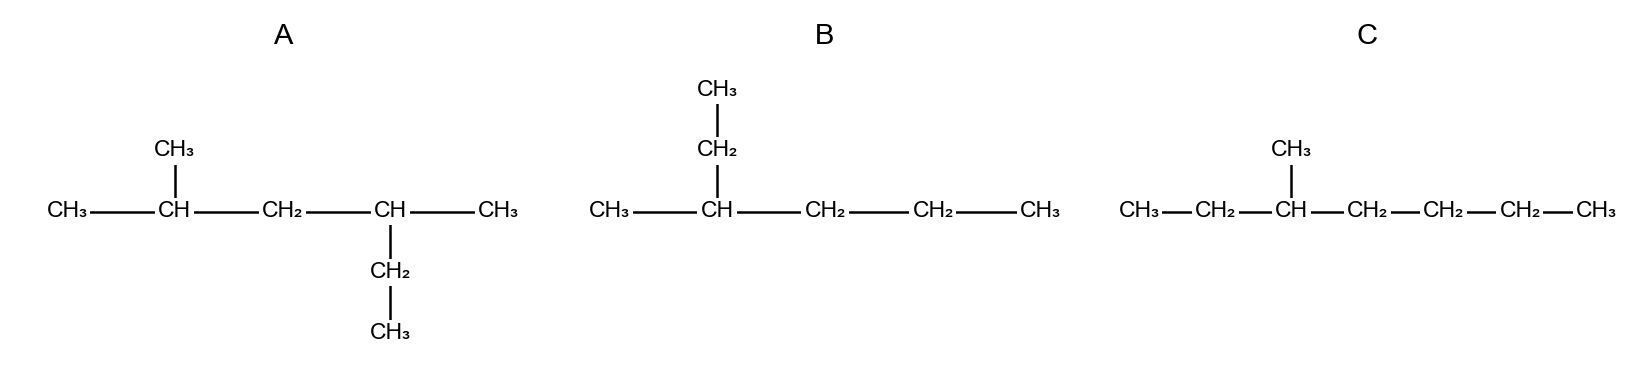
\includegraphics[width=0.86\linewidth]{rasmlar/gen/is_891021.png}\end{center}
Qaysi juftlik o`zaro izomerlar hisoblanadi?

\noindent A)~\textsl{A va B} \hfill B)~\textsl{B va C} \hfill C)~\textsl{A va C} \hfill D)~\textsl{A, B va C}\par
\vspace{4pt}
\end{multicols}
\noindent\textbf{31.} Uch probirkada (\textit{X}, \textit{Y}, \textit{Z}) glitserin, etanol va formalin eritmalari bor. Ularga yangi cho`ktirilgan Cu(OH)\textsubscript{2} ta'sir ettirildi. Kuzatuvlar jadvalda:
\begin{center}
\renewcommand{\arraystretch}{1.15}
\begin{tabular}{|c|c|c|}\hline
\textbf{Probirka} & \textbf{Cu(OH)\textsubscript{2} (sovuqda)} & \textbf{Cu(OH)\textsubscript{2} (qizdirilganda)} \\ \hline
\textit{X} & tiniq ko`k eritma & o`zgarish yo`q \\ \hline
\textit{Y} & o`zgarish yo`q & o`zgarish yo`q \\ \hline
\textit{Z} & o`zgarish yo`q & qizil cho`kma \\ \hline
\end{tabular}
\end{center}
\textit{X}, \textit{Y}, \textit{Z} probirkalardagi \textbf{moddalarni aniqlang.}
\noindent A)~\textsl{\textit{X} -- glitserin, \textit{Y} -- etanol, \textit{Z} -- formalin}\par
\noindent B)~\textsl{\textit{X} -- glitserin, \textit{Y} -- formalin, \textit{Z} -- etanol}\par
\noindent C)~\textsl{\textit{X} -- etanol, \textit{Y} -- glitserin, \textit{Z} -- formalin}\par
\noindent D)~\textsl{\textit{X} -- formalin, \textit{Y} -- etanol, \textit{Z} -- glitserin}\par
\vspace{4pt}
\begin{multicols}{2}
\noindent\textbf{32.} Konsentrlangan sulfat kislotadan suyultirilgan eritma tayyorlashda qanday amal bajariladi?
\noindent A)~\textsl{kislota qizdirilib suvga solinadi}\par
\noindent B)~\textsl{suv kislotaga tez quyiladi}\par
\noindent C)~\textsl{kislota suvga ohista, aralashtirib quyiladi}\par
\noindent D)~\textsl{ikkalasi bir vaqtda quyiladi   ---}\par
\vspace{4pt}
\end{multicols}
\medskip
\noindent\setlength{\fboxsep}{0pt}\fbox{\begin{tabular}{p{0.74\linewidth}|p{0.2\linewidth}}
\parbox[t]{0.72\linewidth}{\vspace{3pt}\textbf{Topshiriqlar (33--35) va javob variant (A--F)larini o`zaro to`g`ri moslashtiring.} Na va Na\textsubscript{2}O dan iborat 10,8 g aralashma 100 g suvda to`liq eritildi, bunda 2,24 l (n.sh.) vodorod ajraldi. Hosil bo`lgan eritma sirka kislota bilan to`liq neytrallandi.
\vspace{3pt}} & \parbox[t]{0.19\linewidth}{\vspace{3pt}A~\textsl{14,5}\\[3pt]
B~\textsl{6,2}\\[3pt]
C~\textsl{24}\\[3pt]
D~\textsl{16}\\[3pt]
E~\textsl{12}\\[3pt]
F~\textsl{4,6}}\\ \hline
\parbox[t]{0.72\linewidth}{\vspace{2pt}\textbf{33. Hosil bo`lgan eritmadagi NaOH ning massa ulushini (\%) aniqlang.}\vspace{2pt}} & \\ \hline
\parbox[t]{0.72\linewidth}{\vspace{2pt}\textbf{34. Dastlabki aralashmadagi Na\textsubscript{2}O massasini (g) aniqlang.}\vspace{2pt}} & \\ \hline
\parbox[t]{0.72\linewidth}{\vspace{2pt}\textbf{35. Neytrallash uchun sarflangan sirka kislota massasini (g) aniqlang.}\vspace{2pt}} & 
\end{tabular}}
\par\bigskip
\noindent\textbf{36.} K\textsubscript{2}Cr\textsubscript{2}O\textsubscript{7} + FeSO\textsubscript{4} + H\textsubscript{2}SO\textsubscript{4} $\to$ Cr\textsubscript{2}(SO\textsubscript{4})\textsubscript{3} + Fe\textsubscript{2}(SO\textsubscript{4})\textsubscript{3} + K\textsubscript{2}SO\textsubscript{4} + H\textsubscript{2}O reaksiya tenglamasini eng kichik butun sonlarda tenglang va barcha koeffitsiyentlar \textbf{yig`indisini aniqlang.}
\javob
\noindent\textbf{37.} Tuzning eruvchanligi 60 \textdegree{}C da 100 g, 20 \textdegree{}C da 20 g (100 g suvda). 60 \textdegree{}C da to`yingan 250 g eritma 20 \textdegree{}C gacha sovitilganda necha gramm tuz cho`kmaga tushadi?
\javob
\noindent\textbf{38.} Zn va ZnO dan iborat 14,6 g aralashma mo`l NaOH eritmasida eritilganda 2,24 l (n.sh.) vodorod ajraldi. Aralashmadagi ZnO \textbf{massasini (g) aniqlang.}
\javob
\noindent\textbf{39.} To`yingan uglevodorod to`liq yondirilganda hosil bo`lgan CO\textsubscript{2} va H\textsubscript{2}O ning mol nisbati 3 : 4 ga teng. Uglevodorodning molyar \textbf{massasini (g/mol) aniqlang.}
\javob
\noindent\textbf{40.} To`yingan bir atomli karbon kislotaning 7,4 g massasi mo`l NaHCO\textsubscript{3} eritmasi bilan reaksiyaga kirishganda 2,24 l (n.sh.) CO\textsubscript{2} ajraldi. Kislotaning molyar \textbf{massasini (g/mol) aniqlang.}
\javob
\par\bigskip\begin{center}\textbf{\fontsize{13}{15}\selectfont YOZMA ISH}\end{center}
\noindent\textbf{41.} \textbf{Topshiriqni bajarish jarayonida barcha reaksiya tenglamalarini yozing. Miqdoriy va arifmetik hisoblashlarni (unga asos bo`lgan usul yoki formulani ko`rsatgan holda) uzviy ketma-ketlikda bajaring.}\par\smallskip
CuSO\textsubscript{4}$\cdot$5H\textsubscript{2}O va Na\textsubscript{2}SO\textsubscript{4}$\cdot$10H\textsubscript{2}O dan iborat 57,2 g aralashma suvda eritilib, 400 g eritma tayyorlandi. Eritma inert elektrodlar yordamida 5 A tok kuchi bilan 3860 s elektroliz qilindi; shu vaqt tugaganda eritmadagi Cu\textsuperscript{2+} ionlari to`liq tugagan edi.\par
\noindent 1)Aralashmadagi kristallogidratlarning massalarini (g) aniqlang.\par
\noindent 2)Dastlabki eritmada CuSO\textsubscript{4} va Na\textsubscript{2}SO\textsubscript{4} ning massa ulushlarini (\%) toping.\par
\noindent 3)Anodda ajralgan gazning hajmini (l, n.sh.) va elektroliz tugagandan keyingi eritma massasini (g) aniqlang.\par
\noindent 4)Elektroliz tugagach eritmadagi H\textsubscript{2}SO\textsubscript{4} va Na\textsubscript{2}SO\textsubscript{4} ning massa ulushlarini (\%) hisoblang.\par
\noindent 5)Shu eritmani to`liq neytrallash uchun zichligi 1,22 g/ml bo`lgan 20\% li NaOH eritmasidan necha ml kerak?\par
\diqqat{Mazkur topshiriq kengaytirilgan javobni talab etib, uning yechilish usuli va shu usul asosidagi barcha hisoblash amallari javoblar varaqasida aks etishi lozim.}
\noindent\textbf{42.} Reaksiya tenglamalarini tugallang va tenglang. Hosil bo`lgan organik moddalarning tuzilish formulalarini yozing va ularni nomlang.\par
\noindent 1)C\textsubscript{2}H\textsubscript{5}Br + KOH(spirtli eritma) $\to$\par
\noindent 2)CH\textsubscript{3}--C$\equiv$CH + H\textsubscript{2}O $\xrightarrow{\text{Hg\textsuperscript{2+}}}$\par
\noindent 3)C\textsubscript{6}H\textsubscript{6} + HNO\textsubscript{3} $\xrightarrow{\text{H\textsubscript{2}SO\textsubscript{4}}}$\par
\noindent 4)CH\textsubscript{3}--CHO + Ag\textsubscript{2}O $\xrightarrow{\text{NH\textsubscript{3}, t}}$\par
\noindent 5)CH\textsubscript{3}COOCH\textsubscript{3} + NaOH $\xrightarrow{\text{t}}$\par
\noindent 6)H\textsubscript{2}N--CH\textsubscript{2}--COOH + NaOH $\to$\par
\noindent 7)n CH\textsubscript{2}=CH--CH=CH\textsubscript{2} $\to$\par
\diqqat{Mazkur topshiriq kengaytirilgan javobni talab etib, uning yechilish usuli va shu usul asosidagi barcha hisoblash amallari javoblar varaqasida aks etishi lozim.}
\noindent\textbf{43.} \textbf{Topshiriqni bajarish jarayonida barcha reaksiya tenglamalarini yozing. Miqdoriy va arifmetik hisoblashlarni (unga asos bo`lgan usul yoki formulani ko`rsatgan holda) uzviy ketma-ketlikda bajaring.}\par\smallskip
37,6 g Cu(NO\textsubscript{3})\textsubscript{2} qizdirilganda qisman parchalandi va qattiq qoldiq massasi 26,8 g bo`ldi. Ajralgan gazlar aralashmasi 200 g suvga to`liq yuttirildi. Qattiq qoldiq esa CuO ni to`liq eritadigan (ortiqcha bo`lmagan) miqdordagi suyultirilgan H\textsubscript{2}SO\textsubscript{4} da eritildi, hosil bo`lgan eritmaga temir qipig`i solindi.\par
\noindent 1)Parchalanish reaksiyasi tenglamasini yozing. Parchalangan Cu(NO\textsubscript{3})\textsubscript{2} ning ulushini (\%) va ajralgan gazlar hajmini (l, n.sh.) aniqlang.\par
\noindent 2)Qattiq qoldiqdagi CuO ning massa ulushini (\%) hisoblang.\par
\noindent 3)Gazlar suvga yuttirilganda hosil bo`lgan eritmadagi HNO\textsubscript{3} ning massa ulushini (\%) toping (reaksiya tenglamasini yozing).\par
\noindent 4)Temir qipig`i eritmadagi barcha Cu\textsuperscript{2+} ionlarini siqib chiqarishi uchun zarur temir massasini (g) va ajralgan mis massasini (g) aniqlang (reaksiya tenglamalarini yozing).\par
\diqqat{Mazkur topshiriq kengaytirilgan javobni talab etib, uning yechilish usuli va shu usul asosidagi barcha hisoblash amallari javoblar varaqasida aks etishi lozim.}
\newpage
\noindent\textbf{\fontsize{13}{15}\selectfont Nazorat testi}\ \textit{$\cdot$ 3-variant}\hfill \textbf{Javoblar kaliti}\par\smallskip\hrule\smallskip
\textit{Faqat o`qituvchi uchun.}\par\medskip
\noindent\textbf{1--32-savollar}\par\smallskip
\noindent\begin{tabular}{|c|c|c|c|c|c|c|c|c|c|c|c|c|c|c|c|}\hline
\textbf{1} & \textbf{2} & \textbf{3} & \textbf{4} & \textbf{5} & \textbf{6} & \textbf{7} & \textbf{8} & \textbf{9} & \textbf{10} & \textbf{11} & \textbf{12} & \textbf{13} & \textbf{14} & \textbf{15} & \textbf{16}\\\hline
\textsl{C} & \textsl{B} & \textsl{B} & \textsl{C} & \textsl{D} & \textsl{B} & \textsl{A} & \textsl{D} & \textsl{D} & \textsl{A} & \textsl{B} & \textsl{B} & \textsl{C} & \textsl{D} & \textsl{B} & \textsl{D}\\\hline
\textbf{17} & \textbf{18} & \textbf{19} & \textbf{20} & \textbf{21} & \textbf{22} & \textbf{23} & \textbf{24} & \textbf{25} & \textbf{26} & \textbf{27} & \textbf{28} & \textbf{29} & \textbf{30} & \textbf{31} & \textbf{32}\\\hline
\textsl{D} & \textsl{C} & \textsl{A} & \textsl{C} & \textsl{A} & \textsl{D} & \textsl{A} & \textsl{A} & \textsl{B} & \textsl{B} & \textsl{D} & \textsl{A} & \textsl{C} & \textsl{C} & \textsl{A} & \textsl{C}\\\hline
\end{tabular}\par\medskip
\noindent\textbf{33--35-savollar}\par\smallskip
\noindent\begin{tabular}{|c|c|c|}\hline \textbf{No} & \textbf{Javob} & \textbf{Qiymat}\\\hline
33 & \textsl{A} & 14,5\\\hline
34 & \textsl{B} & 6,2\\\hline
35 & \textsl{C} & 24\\\hline
\end{tabular}\par\medskip
\noindent\textbf{36--40-savollar}\par\smallskip
\noindent\begin{tabular}{|c|c|}\hline \textbf{No} & \textbf{To`g`ri javob}\\\hline
36 & 26\\\hline
37 & 100\\\hline
38 & 8,1\\\hline
39 & 44\\\hline
40 & 74\\\hline
\end{tabular}\par\medskip
\noindent\textbf{41--43-topshiriqlar: qisqa yechim}\par\smallskip
\noindent\textbf{41-topshiriq.}\par
\noindent 1) Q = 5 $\cdot$ 3860 = 19300 C = 0,2 mol e\textsuperscript{$-$}; Cu\textsuperscript{2+} + 2e\textsuperscript{$-$} $\to$ Cu: n(Cu\textsuperscript{2+}) = 0,1 mol $\to$ CuSO\textsubscript{4}$\cdot$5H\textsubscript{2}O 0,1 mol = 0,1 $\cdot$ 250 = \textbf{25 g}; Na\textsubscript{2}SO\textsubscript{4}$\cdot$10H\textsubscript{2}O = 57,2 $-$ 25 = \textbf{32,2 g} (0,1 mol).\par
\noindent 2) CuSO\textsubscript{4} 0,1 mol = 16 g $\to$ 16/400 = \textbf{4\%}; Na\textsubscript{2}SO\textsubscript{4} 0,1 mol = 14,2 g $\to$ 14,2/400 = \textbf{3,55\%}.\par
\noindent 3) Anod: 2H\textsubscript{2}O $-$ 4e\textsuperscript{$-$} $\to$ O\textsubscript{2} + 4H\textsuperscript{+}; n(O\textsubscript{2}) = 0,2/4 = 0,05 mol $\to$ \textbf{1,12 l}. Eritma massasi: 400 $-$ 6,4 (Cu) $-$ 1,6 (O\textsubscript{2}) = \textbf{392 g}.\par
\noindent 4) 2CuSO\textsubscript{4} + 2H\textsubscript{2}O $\to$ 2Cu + O\textsubscript{2} + 2H\textsubscript{2}SO\textsubscript{4}: H\textsubscript{2}SO\textsubscript{4} 0,1 mol = 9,8 g $\to$ 9,8/392 = \textbf{2,5\%}; Na\textsubscript{2}SO\textsubscript{4} 14,2/392 = \textbf{3,62\%}.\par
\noindent 5) H\textsubscript{2}SO\textsubscript{4} + 2NaOH $\to$ Na\textsubscript{2}SO\textsubscript{4} + 2H\textsubscript{2}O: NaOH 0,2 mol = 8 g; eritma 8/0,2 = 40 g; \textit{V} = 40/1,22 = \textbf{32,8 ml}.\par
\noindent Jami: M 15 + A 10 = 25 ball.\par
\noindent\textbf{42-topshiriq.}\par
\noindent 1) (4 ball) C\textsubscript{2}H\textsubscript{5}Br + KOH(spirt) $\to$ CH\textsubscript{2}=CH\textsubscript{2} + KBr + H\textsubscript{2}O --- etilen (eten).\par
\noindent 2) (4 ball) CH\textsubscript{3}--C$\equiv$CH + H\textsubscript{2}O $\xrightarrow{\text{Hg\textsuperscript{2+}}}$ CH\textsubscript{3}--CO--CH\textsubscript{3} --- propanon (aseton).\par
\noindent 3) (3 ball) C\textsubscript{6}H\textsubscript{6} + HNO\textsubscript{3} $\xrightarrow{\text{H\textsubscript{2}SO\textsubscript{4}}}$ C\textsubscript{6}H\textsubscript{5}NO\textsubscript{2} + H\textsubscript{2}O --- nitrobenzol.\par
\noindent 4) (4 ball) CH\textsubscript{3}CHO + Ag\textsubscript{2}O $\xrightarrow{\text{NH\textsubscript{3}, t}}$ CH\textsubscript{3}COOH + 2Ag$\downarrow$ --- etan (sirka) kislota.\par
\noindent 5) (4 ball) CH\textsubscript{3}COOCH\textsubscript{3} + NaOH $\xrightarrow{\text{t}}$ CH\textsubscript{3}COONa + CH\textsubscript{3}OH --- natriy atsetat va metanol.\par
\noindent 6) (3 ball) H\textsubscript{2}N--CH\textsubscript{2}--COOH + NaOH $\to$ H\textsubscript{2}N--CH\textsubscript{2}--COONa + H\textsubscript{2}O --- glitsinning natriyli tuzi.\par
\noindent 7) (3 ball) n CH\textsubscript{2}=CH--CH=CH\textsubscript{2} $\to$ (--CH\textsubscript{2}--CH=CH--CH\textsubscript{2}--)n --- polibutadiyen.\par
\noindent Jami 4+4+3+4+4+3+3 = 25 ball.\par
\noindent\textbf{43-topshiriq.}\par
\noindent 1) 2Cu(NO\textsubscript{3})\textsubscript{2} $\xrightarrow{\text{t}}$ 2CuO + 4NO\textsubscript{2} + O\textsubscript{2}. Massa kamayishi 37,6 $-$ 26,8 = 10,8 g; 1 mol Cu(NO\textsubscript{3})\textsubscript{2} (188 g) parchalanganda 108 g kamayadi $\to$ 0,1 mol parchalangan; boshlang`ich 37,6/188 = 0,2 mol $\to$ \textbf{50\%}. Gazlar: NO\textsubscript{2} 0,2 mol + O\textsubscript{2} 0,05 mol = 0,25 mol $\to$ \textbf{5,6 l}.\par
\noindent 2) CuO 0,1 mol = 8 g; $\omega$ = 8/26,8 = \textbf{29,9\%}.\par
\noindent 3) 4NO\textsubscript{2} + O\textsubscript{2} + 2H\textsubscript{2}O $\to$ 4HNO\textsubscript{3}: 0,2 mol HNO\textsubscript{3} = 12,6 g; eritma 200 + 9,2 (NO\textsubscript{2}) + 1,6 (O\textsubscript{2}) = 210,8 g; $\omega$ = 12,6/210,8 = \textbf{5,98\%}.\par
\noindent 4) CuO + H\textsubscript{2}SO\textsubscript{4} $\to$ CuSO\textsubscript{4} + H\textsubscript{2}O (0,1 mol); eritmada Cu\textsuperscript{2+}: Cu(NO\textsubscript{3})\textsubscript{2} 0,1 + CuSO\textsubscript{4} 0,1 = 0,2 mol. Fe + Cu\textsuperscript{2+} $\to$ Fe\textsuperscript{2+} + Cu: Fe 0,2 mol = \textbf{11,2 g}; Cu 0,2 mol = \textbf{12,8 g}.\par
\noindent Jami: M 15 + A 10 = 25 ball.\par
\end{document}
